% TODO:
% 1) object migration
% 2) fix ozsu 2009 везде, во всех презентациях
% 3) кажестся в списке литературы должно быть: Straube, D. D. and O¨ zsu, M. T. (1995). Query optimization and execution plan generation in object-oriented database systems. IEEE Trans. Knowl. and Data Eng., 7(2):210–227. 589













%%%%%%%%%%%%%%%%%%%%%%%%%%%%%%%%%%%%%%%%%
% Beamer Presentation
% LaTeX Template
% Version 1.0 (10/11/12)
%
% This template has been downloaded from:
% http://www.LaTeXTemplates.com
%
% License:
% CC BY-NC-SA 3.0 (http://creativecommons.org/licenses/by-nc-sa/3.0/)
%
%%%%%%%%%%%%%%%%%%%%%%%%%%%%%%%%%%%%%%%%%

%----------------------------------------------------------------------------------------
%	PACKAGES AND THEMES
%----------------------------------------------------------------------------------------

\documentclass{beamer}

\mode<presentation> {

% The Beamer class comes with a number of default slide themes
% which change the colors and layouts of slides. Below this is a list
% of all the themes, uncomment each in turn to see what they look like.

%\usetheme{default}
%\usetheme{AnnArbor}
%\usetheme{Antibes}
%\usetheme{Bergen}
%\usetheme{Berkeley}
%\usetheme{Berlin}
%\usetheme{Boadilla}
%\usetheme{CambridgeUS}
%\usetheme{Copenhagen}
%\usetheme{Darmstadt}
%\usetheme{Dresden}
%\usetheme{Frankfurt}
%\usetheme{Goettingen}
%\usetheme{Hannover}
%\usetheme{Ilmenau}
%\usetheme{JuanLesPins}
%\usetheme{Luebeck}
\usetheme{Madrid}
%\usetheme{Malmoe}
%\usetheme{Marburg}
%\usetheme{Montpellier}
%\usetheme{PaloAlto}
%\usetheme{Pittsburgh}
%\usetheme{Rochester}
%\usetheme{Singapore}
%\usetheme{Szeged}
%\usetheme{Warsaw}

% As well as themes, the Beamer class has a number of color themes
% for any slide theme. Uncomment each of these in turn to see how it
% changes the colors of your current slide theme.

%\usecolortheme{albatross}
%\usecolortheme{beaver}
%\usecolortheme{beetle}
%\usecolortheme{crane}
%\usecolortheme{dolphin}
%\usecolortheme{dove}
%\usecolortheme{fly}
%\usecolortheme{lily}
%\usecolortheme{orchid}
%\usecolortheme{rose}
%\usecolortheme{seagull}
%\usecolortheme{seahorse}
%\usecolortheme{whale}
%\usecolortheme{wolverine}

%\setbeamertemplate{footline} % To remove the footer line in all slides uncomment this line
%\setbeamertemplate{footline}[page number] % To replace the footer line in all slides with a simple slide count uncomment this line

%\setbeamertemplate{navigation symbols}{} % To remove the navigation symbols from the bottom of all slides uncomment this line
}

\usepackage[utf8]{inputenc}
\usepackage[russian]{babel}
\usepackage{cmap}


\usepackage{verbatim}
\usepackage{fancybox}
\usepackage{ulem}
\usepackage{tikz}
\usetikzlibrary{positioning}
\usepackage{scalefnt}
\usetikzlibrary{arrows,shapes,positioning,shadows,trees,calc,backgrounds,fit,positioning}

\usepackage{graphicx} % Allows including images
\usepackage{booktabs} % Allows the use of \toprule, \midrule and \bottomrule in tables
\usepackage{textcomp}
\usepackage{listings}
\usepackage{color}
\usepackage{xcolor}
\usepackage{changepage}

\definecolor{mygreen}{rgb}{0,0.6,0}
\definecolor{mygray}{rgb}{0.5,0.5,0.5}
\definecolor{mymauve}{rgb}{0.58,0,0.82}

\lstset{ %
  backgroundcolor=\color{white},   % choose the background color; you must add \usepackage{color} or \usepackage{xcolor}
  basicstyle=\footnotesize,        % the size of the fonts that are used for the code
  breakatwhitespace=false,         % sets if automatic breaks should only happen at whitespace
  breaklines=true,                 % sets automatic line breaking
  captionpos=b,                    % sets the caption-position to bottom
  commentstyle=\color{mygreen},    % comment style
  deletekeywords={...},            % if you want to delete keywords from the given language
  escapeinside={\%*}{*)},          % if you want to add LaTeX within your code
  extendedchars=true,              % lets you use non-ASCII characters; for 8-bits encodings only, does not work with UTF-8
  frame=single,                    % adds a frame around the code
  keepspaces=true,                 % keeps spaces in text, useful for keeping indentation of code (possibly needs columns=flexible)
  keywordstyle=\color{blue},       % keyword style
  language=Octave,                 % the language of the code
  morekeywords={*,...},            % if you want to add more keywords to the set
  numbers=left,                    % where to put the line-numbers; possible values are (none, left, right)
  numbersep=5pt,                   % how far the line-numbers are from the code
  numberstyle=\tiny\color{mygray}, % the style that is used for the line-numbers
  rulecolor=\color{black},         % if not set, the frame-color may be changed on line-breaks within not-black text (e.g. comments (green here))
  showspaces=false,                % show spaces everywhere adding particular underscores; it overrides 'showstringspaces'
  showstringspaces=false,          % underline spaces within strings only
  showtabs=true,                  % show tabs within strings adding particular underscores
  stepnumber=1,                    % the step between two line-numbers. If it's 1, each line will be numbered
  stringstyle=\color{mymauve},     % string literal style
  tabsize=4,                       % sets default tabsize to 2 spaces
  %title=\lstname                   % show the filename of files included with \lstinputlisting; also try caption instead of title
}

\graphicspath{{./figures/}}

%----------------------------------------------------------------------------------------
%	TITLE PAGE
%----------------------------------------------------------------------------------------

\title[Обработка и исполнение запросов: лекция 10]{Обработка и исполнение запросов в СУБД (Лекция 10) \\~\\ Объектные и Объектно-Реляционные СУБД\\~\\ v5} % The short title appears at the bottom of every slide, the full title is only on the title page

\author{Георгий Чернышев} % Your name
\institute[ВШЭ] % Your institution as it will appear on the bottom of every slide, may be shorthand to save space
{
Высшая Школа Экономики \\ % Your institution for the title page
\medskip
\textit{chernishev@gmail.com} % Your email address
}
%\date{\today} % Date, can be changed to a custom date

\date{25 ноября 2020 г.}

\begin{document}

\begin{frame}
\titlepage % Print the title page as the first slide
\end{frame}

\begin{comment}
\begin{frame}
\frametitle{Overview} % Table of contents slide, comment this block out to remove it
\tableofcontents % Throughout your presentation, if you choose to use \section{} and \subsection{} commands, these will automatically be printed on this slide as an overview of your presentation
\end{frame}
\end{comment}

\begin{frame}
\frametitle{План}

\begin{itemize}
  %\setlength\itemsep{1em}
  \item Объектные модели: 
  \begin{enumerate}
    \item Объектно-ориентированная База Данных;
    \item Объектно-реляционная База Данных;
  \end{enumerate}
  \item Вопросы архитектуры ОСУБД:
  \begin{enumerate}
    \item Клиент-сервер: объектный и страничный вариант;
    \item Управление буфером;
    \item Управление OID;
    \item Pointer Swizzling;
    \item Исполнение запросов.
  \end{enumerate}
\end{itemize}
\end{frame}

\begin{frame}
\frametitle{Объектные модели \cite{{Urban2009}}}

\begin{itemize}
  %\setlength\itemsep{1em}
  \item Реляционная модель не всегда подходит (в нишевых системах~--- CAD, OIS, ...) \cite{Ozsu2011}: 
  \begin{enumerate}
    \item Иногда нужна возможность задавать пользовательские типы данных (application-specific data types);
    \item Пологая структура иногда плоха, иногда нужно отражать отношение включения что сложно сделать в реляционной модели;
    \item Реш. проблемы несоответствия импеданса (impedance mismatch);
  \end{enumerate}
  \item Object-Oriented Database System (OODB):
  \begin{enumerate}
    \item Object-Oriented Database System Manifesto, середина 1980-х;
    \item Классы, иерархии, OID-ы;
    \item OOPL~--- единый язык для доступа в базу и разработки приложения, импеданса нет;
  \end{enumerate}

  \item Object-Relational Database (ORDB):
  \begin{enumerate}
    \item Third generation database system manifesto, 1990-ый;
    \item Первая ORDB~--- Postgres \cite{Rowe1987}; 
    \item UDT, таблицы из объектов, ID у записей;
  \end{enumerate}

\end{itemize}
\end{frame}

\begin{frame}
\frametitle{Объектная модель, основы \cite{Urban2009}}

\begin{itemize}
  \setlength\itemsep{1em}
  \item Сущности представляются объектами, имеют состояние и поведение;
  \item Состояние~--- набор структурных свойств объекта;
  \item Поведение описывается через методы;
  \item Объекты с одинаковым интерфейсом объединяются в класс;
  \item Каждый объект класса получает уникальный внутрениий идентификатор~--- OID,  он иммутабелен;
  \item Связи между объектами реализуются с помощью ссылок;
  \item Классы можно объединять в иерархии, наследование;
\end{itemize}
\end{frame}


\begin{frame}[t]
\frametitle{Пример: объектная модель данных, UML}

\begin{figure}[htb]
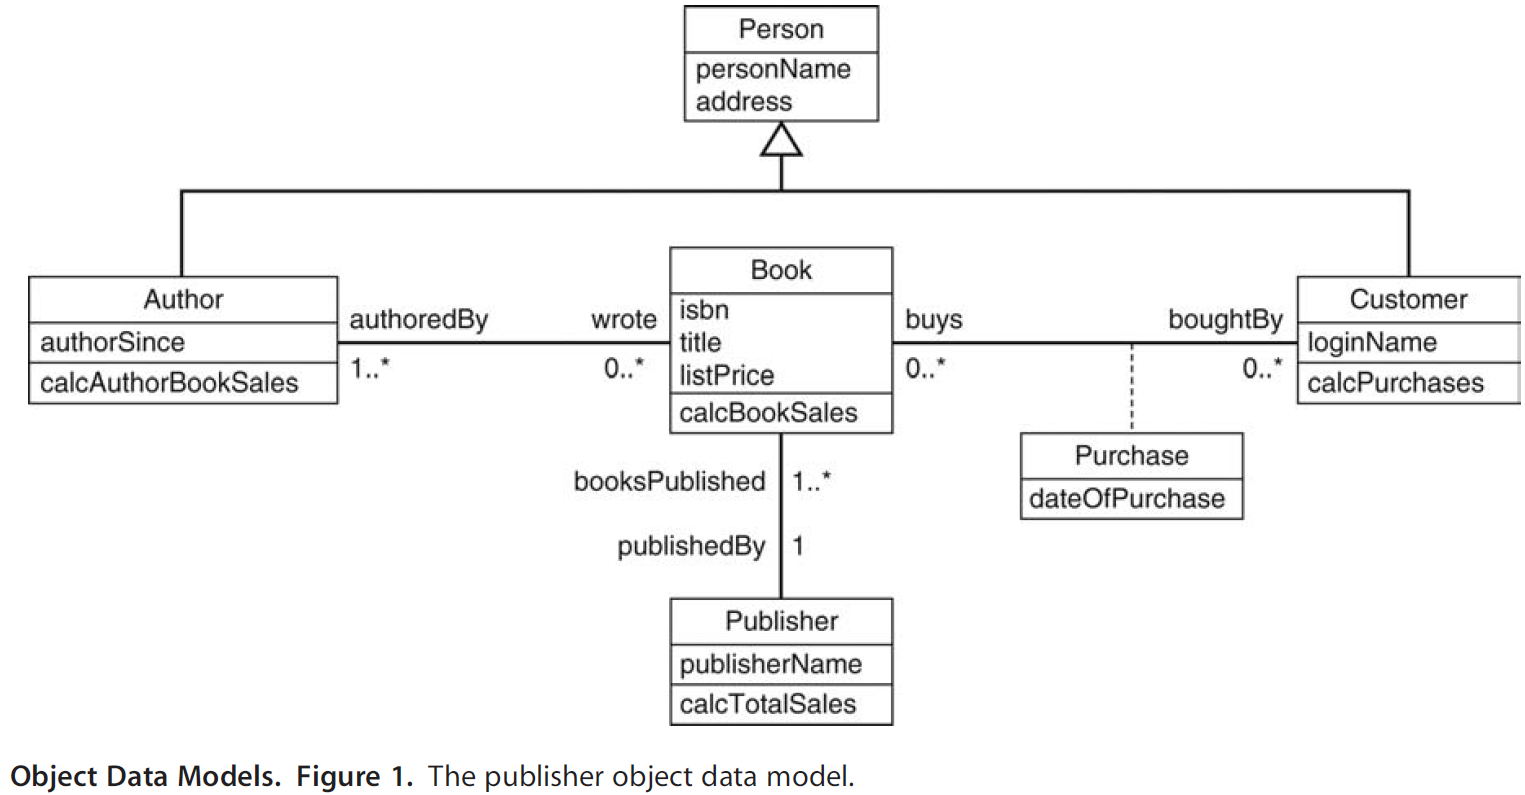
\includegraphics[width=\textwidth,height=0.77\textheight,keepaspectratio]{object-data-model.png} 
\footnote{\tiny{Изображение взято из \cite{Urban2009}}}
\end{figure}    
  
\end{frame}

\begin{frame}
\frametitle{Объектно-Ориентированная модель \cite{{Urban2009}}}

\begin{itemize}
  \setlength\itemsep{1em}
  \item Суть OODB: база данных в которой объект это основная единица работы, плюс есть некоторый ОО язык для запросов;
  \item Object Data Standard~--- содержит описание модели, язык задания схемы (ODL), язык запросов (OQL), разработан ODMG \cite{Ozsu2011};
  \item ODL (Object Definition Language) ~--- язык спецификации объектной схемы: задание свойств объектов и сигнатур методов;
  \item Свойство это атрибут или отношение между объектами;
  \item В ODL отношения одно или двунаправленные (тогда СУБД поддерживает целостность);
  
\end{itemize}
\end{frame}

\begin{frame}[t]
\frametitle{Пример: ОО модель данных, OODB Schema, ODL}

\begin{figure}[htb]
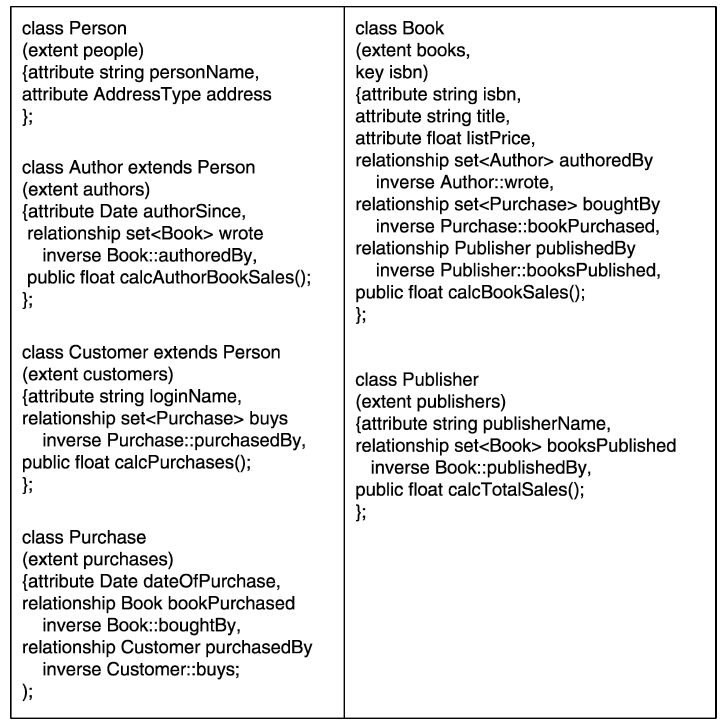
\includegraphics[width=\textwidth,height=0.77\textheight,keepaspectratio]{object-oriented-data-model.png} 
\footnote{\tiny{Изображение взято из \cite{Urban2009}}}
\end{figure}    
  
\end{frame}

\begin{frame}[t]
\frametitle{Пример: ОО модель данных, OODB Schema, ODL}

\begin{figure}[htb]
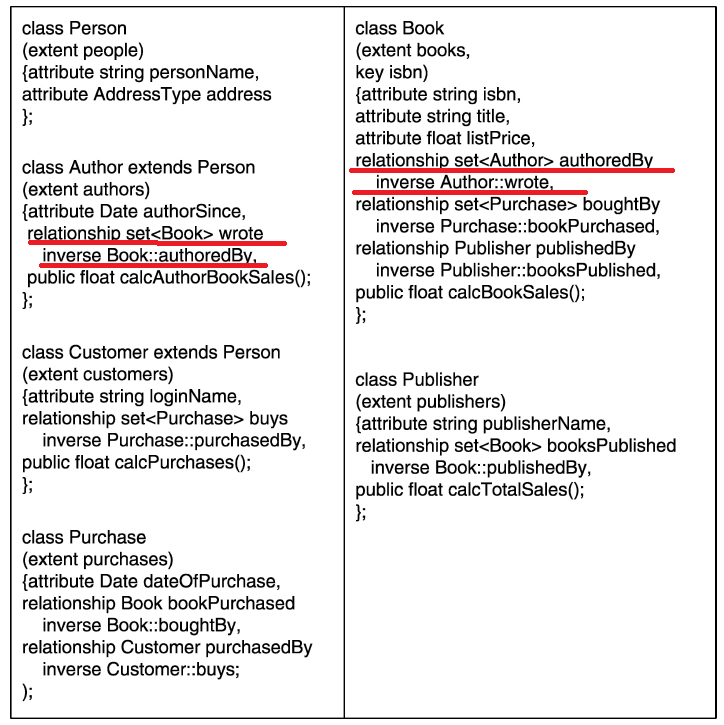
\includegraphics[width=\textwidth,height=0.77\textheight,keepaspectratio]{object-oriented-data-model2.png} 
\footnote{\tiny{Изображение взято из \cite{Urban2009}}}
\end{figure}    
  
\end{frame}


\begin{frame}[fragile]
\frametitle{ОО модель \cite{{Urban2009}}}

Замечания по языкам:

\lstset{language=SQL}

\begin{itemize}
  %\setlength\itemsep{1em}
  \item Можно задавать объектную схему на некотором OOPL, поддерживающимся в СУБД: C++, Java, ...
  \item Описание схемы и реализация методов на некотором языке называется language binding;
  \item Стандарт ODL говорит и о Object Query Language (OQL), подобие SQL, но можно ``ходить'' по ``.'' и вызывать методы:
  \begin{lstlisting}
    select b.publishedBy.publisherName
    from books b
    where b.isbn = ``0-13-042898-1'';\end{lstlisting}

  \begin{lstlisting}
    select title: b.title, sales: b.calcBookSales()
    from p in publishers, b in p.booksPublished
    where p.publisherName = ``Springer-Verlag'' \end{lstlisting}
            
\end{itemize}
\end{frame}

\begin{frame}[fragile]
\frametitle{Объектно-Реляционная модель \cite{{Urban2009}}}
\lstset{language=SQL}
\begin{itemize}
  \setlength\itemsep{1em}
  \item Суть OORB: расширение реляционных СУБД, добавили типизированную таблицу (подобна классу в OODB), основана на UDT;  
  \item Стандарт предложен в SQL3 (SQL1999);
  \item Можно иметь иерархии объектов;
  \item У записи (у объекта) такой таблицы есть OID;
  \item Ссылки в объектах по OID задают отношения между объектами:
    \begin{enumerate}
    \item scope указывает на таблицу;
    \item refs are checked~--- аналог ссылочной целостности, триггеров;
    \end{enumerate}
\end{itemize}
\end{frame}

\begin{frame}[t]
\frametitle{Пример: О-Р модель данных, ORDB Schema, SQL Stan-d}

\begin{figure}[htb]
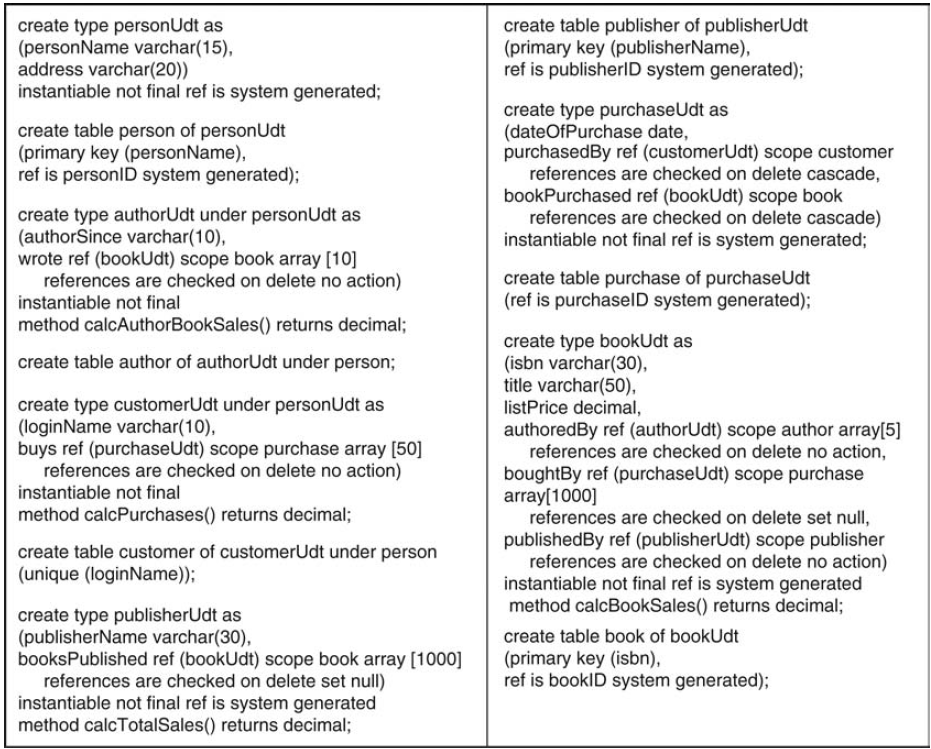
\includegraphics[width=\textwidth,height=0.77\textheight,keepaspectratio]{object-relational-data-model.png} 
\footnote{\tiny{Изображение взято из \cite{Urban2009}}}
\end{figure}      
\end{frame}

\begin{frame}[t]
\frametitle{Пример: О-Р модель данных, ORDB Schema, SQL Stan-d}

\begin{figure}[htb]
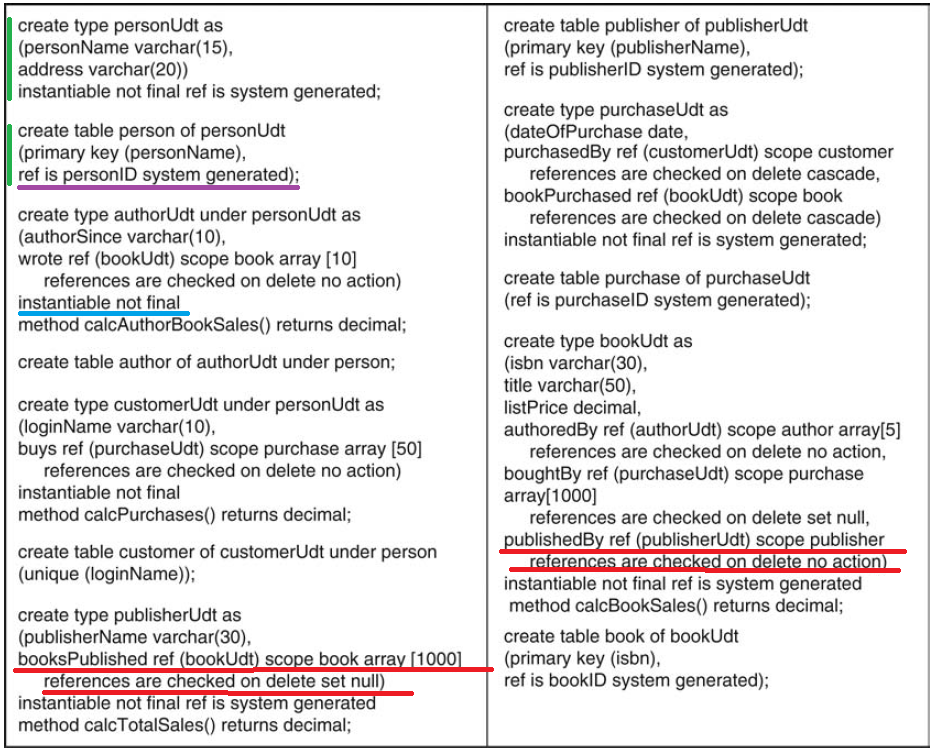
\includegraphics[width=\textwidth,height=0.77\textheight,keepaspectratio]{object-relational-data-model2.png} 
\footnote{\tiny{Изображение взято из \cite{Urban2009}}}
\end{figure}      
\end{frame}

\begin{frame}[fragile]
\frametitle{Запросы в ОР модели \cite{{Urban2009}}}
\lstset{language=SQL}
\begin{itemize}
  %\setlength\itemsep{1em}
  \item Запрос, прописываем OID:    
  \begin{lstlisting}
  update book set publishedBy = 
    (select publisherID from publisher
      where publisherName =``Prentice Hall'')
  where isbn = ``0-13-042898-1'';\end{lstlisting}
  \item По точкам тоже можно ходить (там скрыт join):
  \begin{lstlisting}
  select publishedBy.publisherName
  from book
  where isbn = ``0-13-042898-1'';\end{lstlisting}
  \item Можно разыменовать указатель:
  \begin{lstlisting}
    select deref(publishedBy)
    from book
    where isbn = ``0-13-042898-1'';\end{lstlisting}

\end{itemize}
\end{frame}

\begin{frame}
\frametitle{Замечание}

Если кому-то нужно полноценное введение в объекты \alert{с оглядкой на базы данных}, то есть, не ясны понятия: объект, тип, класс, подкласс, наследование, композиция то читайте 15.1 (Distributed Object Database Management) из \cite{Ozsu2011}.

\end{frame}

\begin{frame}
\frametitle{Вопросы архитектуры распределенных ОСУБД по \"{O}zsu}

Много всего:

\begin{itemize}
  \setlength\itemsep{1em}
  \item Варианты клиент/серверной архитектуры;
  \item Управление буфером на клиенте и на сервере;
  \item \alert{Кеши и их консистентность;}
  \item Управление OID-ами;
  \item \alert{Миграция объектов;}
  \item \alert{Кластеризация объектов;}
  \item \alert{Распределенный GC;}
  \item {\color{blue}Обработка и выполнение запросов в OODB.}

\end{itemize}
\end{frame}

\begin{frame}
\frametitle{Отличия ОСУБД от реляционных систем}

Сразу думаем о клиент-серверных системах (лекция 4).
\\~\\
Много аспектов:

\begin{itemize}
  \setlength\itemsep{1em}
  \item Какова будет единица обмена между клиентом и сервером: страница или объект (или группа объектов)?
  \item Какие функции предоставляет клиент, а какие сервер? Объекты не пассивны, может быть активное взаимодействие которое полезно пооптимизировать.
  \item В реляционных системах преобладает function shipping (лекция 5), но в объектных может быть очень полезен data shipping.
  \item В ОСУБД необходим prefetch по данным.
\end{itemize}

Итог~--- два подхода: объектные и страничные сервера.

\end{frame}

\begin{frame}[t]
\frametitle{Варианты клиент/серверной архитектуры ОСУБД I}

\begin{figure}[htb]
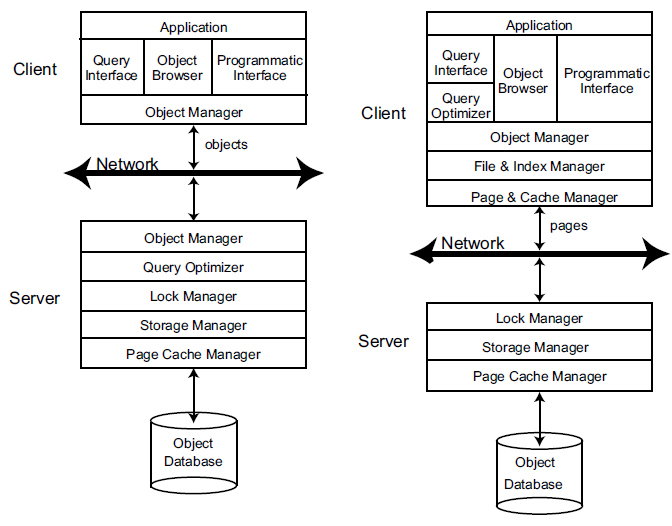
\includegraphics[width=\textwidth,height=0.77\textheight,keepaspectratio]{architectures.png} 
\footnote{\tiny{Изображение взято из \cite{Ozsu2011}}}
\end{figure}      
\end{frame}

\begin{frame}
\frametitle{Варианты клиент/серверной архитектуры ОСУБД II}

В зависимости от гранулярности данных и предоставляемой функциональности бывают:

\begin{itemize}
  %\setlength\itemsep{1em}
  \item Объектные сервера:
  \begin{itemize}
    \item Сервер делает основную работу;
    \item Менеджер объектов (OM) предоставляет контекст для исполнения методов, можно выполнять на сервере и на клиенте;
    \item Управление OID-ом~--- ответственность OM (удаление, GC);
    \item На сервере OM отвечает за кластеризацию;
    \item На клиенте и сервере кеши из объектов, на сервере страничный;
    \item Оптимизацию пользовательских запросов делает сервер, он же синхронизацию транзакций;

  \end{itemize}  
  \item Страничные сервера:
  \begin{itemize}
    \item Можно рассматривать как улучшенный storage manager: базовая единица обмена данными страница или сегмент, а не объект;
  \end{itemize}  

\end{itemize}
\end{frame}

% ^ можно передавать не один объект, а несколько
% тогда проблема: если клиенту приходит обратно измененная версия, надо делать installation read, чтобы записать изменения	


\begin{frame}
\frametitle{Варианты клиент/серверной архитектуры ОСУБД III}

Страничный подход считается лучшим, хотя результаты не финальны, хорошо получалось когда: кластеризация совпадает с паттерном доступа из запроса; когда был \alert{один сервер} и один/несколько клиентов и т.д.

\begin{itemize}
 % \setlength\itemsep{1em}
  \item Страничные сервера:
  \begin{itemize}
    \setlength\itemsep{1em}
    \item Упрощают код СУБД: страничные кеши на клиенте и сервере, единое представление данных вплоть до пользователя;
    \item Обновления просто заливать с клиента на сервер;
    \item Более полное использование ресурсов клиента при выполнении запросов;
    \item Нагрузку можно балансировать с помощью оптимизатора;
    \item Можно эффективно использовать ОС, железо (pointer swizzling);
  \end{itemize}  

\end{itemize}
\end{frame}

\begin{frame}
\frametitle{Варианты клиент/серверной архитектуры ОСУБД IV}

Некоторые соображения на тему:
\begin{itemize}
 % \setlength\itemsep{1em}
  \item Казалось бы, объектная модель по производительности должна иметь преимущества~--- если сервер будет ``понимать'' концепцию объекта:
  \begin{itemize}
    \item Замки и логгирование на уровне объектов, а не страниц;
    \item Фильтрация на сервере: слать меньше + разгрузить клиента;
  \end{itemize}
  \item Фильтрация на сервере не так уж однозначно хороша. Нагрузка это смесь из запросов и пообъектной навигации. Для каждого объекта по вызову RPC~--- плохо (причина победы страничного подхода~--- навигационные тестовые нагрузки).
  \item Возможное решение проблемы навигации: слать код на сервер и там исполнять. Появляется другая проблема: безопасность.
  \item Есть системы умеющие переключаться между режимами: $O_2$.
\end{itemize}
\end{frame}

\begin{frame}
\frametitle{Управление буфером}

\begin{itemize}
 % \setlength\itemsep{1em}
  \item Клиент. Если page fault информация берется с сервера. Бывает:
  \begin{itemize}
    \item Объектный~--- на уровне объекта: (+) высокая гранулярность $\longrightarrow$ высокая конкурентность (-) фрагментация;
    \item Страничный~--- на уровне страницы: (+) нет фрагментации (-) не угадали с шаблоном кластеризации $\longrightarrow$ будем подгружать постоянно;
    
    \item Двойной~--- есть оба, при сбросе страничного, откопируем полезные объекты в объектный. Копим хорошо кластеризованные страницы и объекты.
  \end{itemize}
  \item Сервер. Если случается page fault --- информация берется с диска.
  \begin{itemize}
    \item Аналогичен реляционным в части общения с диском. Если нужны группы объектов, конструирует их из страниц и шлет на клиент.
    \item MOB (Modified Object Buffer)~--- амортизация записи на диск.
    \item LRU hate hints на сервере (разделять информацию на сервере и клиенте, стремиться чтобы всё обслуживалось клиентом).
  \end{itemize}
  
\end{itemize}
\end{frame}


\begin{frame}
\frametitle{Управление OID I}

Как реализовывать постоянный ID объекта? Объекты бывают постоянные, временные, созданные пользователем или системой.

\begin{itemize}
 \setlength\itemsep{1em}
  \item Physical identifier (POID)~--- физический адрес. Стратегия: OID приравниватся к физическому адресу объекта. Например, адрес страницы + смещение.
  \begin{itemize}
    \item (+) Получаем адрес объекта из OID сразу;
    \item (-) ``Родителей'' надо обновлять при переезде на новую страницу;
  \end{itemize}
  \item Logical identifier (LOID)~--- каждому объекту, дается уникальный в рамках системы ID. Бывает:
  \begin{itemize}
    \item Чистый LOID, генерируются с помощью уникального в рамках системы счетчика;
    \item Псевдо LOID, сервер ID сконкатенированный со счетчиком в рамках сервера;
  \end{itemize}
  \item Для стратегии LOID надо держать таблицу трансляции в POID;
  \begin{itemize}
    \item Придется тратить один look-up по таблице  :(
  \end{itemize}
  \item Зато не надо обновлять LOID при перемещении объекта.
\end{itemize}
\end{frame}


\begin{frame}
\frametitle{Управление OID II}

\begin{itemize}
 \setlength\itemsep{1em}
  \item Распределенные объектные системы предпочитают LOID, из-за динамичности окружения в котором работает СУБД;
  \item Трюк: для маленьких значений не разделяемых по ссылке, хранить их значение в OID (меньше таблица, быстрее получение);
  \item Генерация LOID: 
  \begin{itemize}
    \item чистый LOID дорог: сетевые задержки + доп. нагрузка на узел;
    \item номер генерируется секвенцей, не переиспользуется при удалении.
  \end{itemize}
  \item Трансляция LOID-POID: 
  \begin{itemize}
    \item Если чистый LOID и клиент подключен к нескольким серверам то таблица на клиенте;
    \item Если псевдо LOID, то только на серверах;
    \item На клиенте держать нежелательно: не масштабируемо, надо синхронизировать таблицы на всех подключенных клиентах;
    \item Таблица хранится в виде $B^+$-дерева или хеш-таблицы.
  \end{itemize}  
\end{itemize}
\end{frame}

\begin{frame}
\frametitle{Pointer Swizzling I}

При вычислении Path Expressions вида c.engine.manufacturer.name надо подгружать данные с диска. На диске OID, но в памяти лучше использовать указатели. Подход динамической подмена на указатели~--- pointer swizzling (словарь: ``настройка по адресам''). Методы:

\begin{itemize}
 \setlength\itemsep{1em}
  \item Хардварный: если приходит от ОС page fault загружаем страницу, конвертируем на ней все OID в указатели на несуществующие страницы. Резервируем место на эти страницы. Эти страницы подгружаются только когда их, в свою очередь, ``тронут'' (перехватываем page fault от ОС).
  \item Софтварный: используется таблица объектов. Указатель подменяется так, чтобы указывать на место в таблице объектов (LOID).
  \item Бывают eager и lazy софтварные схемы.
\end{itemize}
\end{frame}

\begin{frame}
\frametitle{Pointer Swizzling II}

\begin{itemize}
 \setlength\itemsep{1em}
  \item Хардварный: лучше когда постоянно ходим по одной группе объектов, меньше косвенных обращений (к таблице объектов);
  \item Но! Плохая кластеризация, мало нужных объектов на странице, много перехватов page faults $\longrightarrow$ хардварный будет страдать;
  \item Удаления обрабатывать сложнее, транзакционность сложнее, хардварная ориентирована на страничные сервера;
  \item При хардварной может кончиться память (постоянно резервируем);
  \item При хардварной трудно работать на уровне объектов.
\end{itemize}
\end{frame}



\begin{frame}
\frametitle{Исполнение запросов в ОСУБД \cite{Ozsu2011}}
Базируется на принципах реляционных СУБД, однако есть отличия:
\begin{itemize}
  %\setlength\itemsep{1em}
  \item Более сложная алгебра операций: 
  \begin{itemize}
    \item оперируем над наборами объектов;
    \item наборы семантически разные: список, множество, bag;
    \item $\longrightarrow$ необходим сложный механизм вывода типов.
  \end{itemize}
  \item В реляционных стоимости основываются на AM, физическом расположении данных. Информация легко доступна оптимизатору
  \begin{itemize}
    \item стоимость выполнения методов сложнее оценить;
    \item так как ЯП общего назначения, то методы надо оптимизировать;
    \item инкапсуляция мешает, иногда оптимизатор игнорирует ее.
  \end{itemize}
  \item Сложная (ссылочная) структура на объектах:
  \begin{itemize}
    \item центральная проблема: оптимизация path expressions;
    \item доступ к атрибутам через граф наследования тоже надо оптимизировать.
  \end{itemize}  
\end{itemize}
\end{frame}

\begin{frame}
\frametitle{Оптимизация Path Expressions}

Пример: c.engine.manufacturer.name. Интересные моменты:

\begin{itemize}
 \setlength\itemsep{1em}
  \item Занимались с начала 80-х, проблема: могут быть и методы!
  \item Соединения на графе;
  \item Path index: аналог join index, можно строить не только для цепочки вызовов, но и для графа наследования;
  \item Access support relation: структура данных для хранения избранных path expressions.
\end{itemize}
\end{frame}

\begin{frame}
\frametitle{Про оптимизацию}

Если кому-то интересно про оптимизацию в объектных системах то смотрите \cite{Mitchel1993}, \cite{Ozsu0}, \cite{Straube1987}. 
\\~\\
А начать стоит с дочитывания 15.6 (Distributed Object Database Management) из \cite{Ozsu2011}.

\end{frame}

\begin{comment}

\begin{frame}[t]
\frametitle{Примеры систем}

\begin{figure}[htb]
%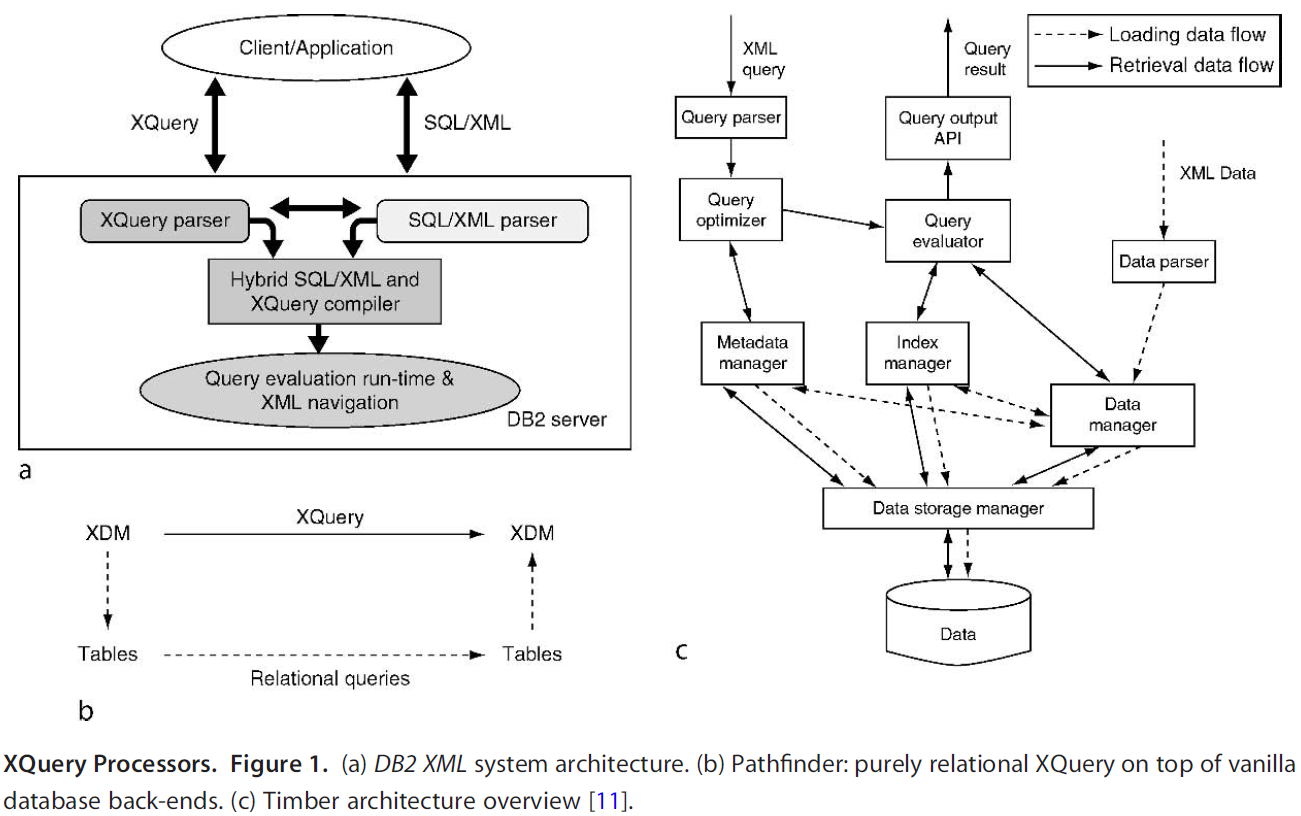
\includegraphics[width=\textwidth,height=0.77\textheight,keepaspectratio]{xml-approaches.png} 
\footnote{\tiny{Изображение взято из \cite{Grust2009}}}
\end{figure}    
  
\end{frame}

\end{comment}

\begin{frame}[allowframebreaks]
\frametitle{Ссылки}
\footnotesize{
\begin{thebibliography}{99}

\bibitem[Mitchel, 1993] {Mitchel1993} Gail Anne Mitchel. Extensible Query Processing in an Object-Oriented Database. Technical Report TR93-16. Department of Computer Science, Brown University. \url{ftp://ftp.cs.brown.edu/pub/techreports/93/cs93-16.pdf}

\bibitem[Ozsu and Blakeley, 1990] {Ozsu0} M. Tamer Özsu and Jose A. Blakeley. Query Processing in Object-Oriented Database Systems. 19 pages. \url{https://cs.uwaterloo.ca/~tozsu/publications/odbms/wonkim/kimchap.pdf}

\bibitem[Straube and Ozsu, 1990] {Straube1987} David D. Straube and M. Tamer Özsu. 1990. Queries and query processing in object-oriented database systems. ACM Trans. Inf. Syst. 8, 4 (October 1990), 387--430. DOI=http://dx.doi.org/10.1145/102675.102678 

\bibitem[Rowe and Stonebraker, 1987] {Rowe1987} Rowe L. and Stonebraker M. The Postgres Data Model. In Proc. 13th Int. Conf. on Very Large Data Bases. 1987.

\bibitem[Urban and Dietrich, 2009] {Urban2009} Susan D. Urban, Suzanne W. Dietrich. Object Data Models. Encyclopedia of Database Systems. Springer US, 2009. 1929--1935. \url{http://dx.doi.org/10.1007/978-0-387-39940-9_249}

%\bibitem[Jagadish et al., 2002] {Jagadish2002} H. V. Jagadish, S. Al-Khalifa, A. Chapman, L. V. S. Lakshmanan, A. Nierman, S. Paparizos, J. M. Patel, D. Srivastava, N. Wiwatwattana, Y. Wu, and C. Yu. 2002. TIMBER: A native XML database. The VLDB Journal 11, 4 (December 2002), 274--291. DOI=http://dx.doi.org/10.1007/s00778-002-0081-x 

%\bibitem[Luna Dong and Srivastava, 2009] {Luna2009} Xin Luna Dong, Divesh Srivastava. XML Indexing. Encyclopedia of Database Systems. Springer US, 2009. 3585--3591. \url{http://dx.doi.org/10.1007/978-0-387-39940-9_779}

%\bibitem[Grust et al., 2009] {Grust2009} Torsten Grust, H. V. Jagadish, Fatma Ozcan, Cong Yu. XQuery Processors. Encyclopedia of Database Systems. Springer US, 2009. 3671--3675.

%\bibitem[Hidders and Paredaens, 2009] {Hidders2009} Jan Hidders and Jan Paredaens. XPath/XQuery. Encyclopedia of Database Systems. Springer US, 2009. 3659--3665.\url{http://dx.doi.org/10.1007/978-0-387-39940-9_774}

%\bibitem[Taranov et al., 2010] {Taranov2010} Ilya Taranov, Ivan Shcheklein, Alexander Kalinin, Leonid Novak, Sergei Kuznetsov, Roman Pastukhov, Alexander Boldakov, Denis Turdakov, Konstantin Antipin, Andrey Fomichev, Peter Pleshachkov, Pavel Velikhov, Nikolai Zavaritski, Maxim Grinev, Maria Grineva, and Dmitry Lizorkin. 2010. Sedna: native XML database management system (internals overview). In Proceedings of the 2010 ACM SIGMOD International Conference on Management of data (SIGMOD '10). ACM, New York, NY, USA, 1037-1046. DOI=http://dx.doi.org/10.1145/1807167.1807282 

%\bibitem[Ivanova et al., 2010] {Ivanova2010} Milena G. Ivanova, Martin L. Kersten, Niels J. Nes, and Romulo A.P. Gonçalves. 2010. An architecture for recycling intermediates in a column-store. ACM Trans. Database Syst. 35, 4, Article 24 (October 2010), 43 pages. DOI=10.1145/1862919.1862921 http://doi.acm.org/10.1145/1862919.1862921 

%\bibitem[Shatdal et al., 1994] {Shatdal1994} Ambuj Shatdal, Chander Kant, and Jeffrey F. Naughton. 1994. Cache Conscious Algorithms for Relational Query Processing. In Proceedings of the 20th International Conference on Very Large Data Bases (VLDB '94), Jorge B. Bocca, Matthias Jarke, and Carlo Zaniolo (Eds.). Morgan Kaufmann Publishers Inc., San Francisco, CA, USA, 510--521. 

%\bibitem[Boncz et al., 2008] {Boncz2008} Peter A. Boncz, Martin L. Kersten, and Stefan Manegold. 2008. Breaking the memory wall in MonetDB. Commun. ACM 51, 12 (December 2008), 77--85. DOI=http://dx.doi.org/10.1145/1409360.1409380 

%\bibitem[Boncz et al., 2005] {Boncz2005} Peter Boncz, Marcin Zukowski, Niels Nes. MonetDB/X100: Hyper-Pipelining Query Execution. CIDR'05.

%\bibitem[Hennessy and Patterson, 2011] {Hennessy2011}  John L. Hennessy and David A. Patterson. 2011. Computer Architecture, Fifth Edition: A Quantitative Approach (5th ed.). Morgan Kaufmann Publishers Inc., San Francisco, CA, USA. 

%\bibitem[Tsirogiannis et al., 2009] {Tsirogiannis2009}  Dimitris Tsirogiannis, Stavros Harizopoulos, Mehul A. Shah, Janet L. Wiener, and Goetz Graefe. 2009. Query processing techniques for solid state drives. In Proceedings of the 2009 ACM SIGMOD International Conference on Management of data (SIGMOD '09), Carsten Binnig and Benoit Dageville (Eds.). ACM, New York, NY, USA, 59-72. DOI=http://dx.doi.org/10.1145/1559845.1559854 

%\bibitem[Li and Ross, 1999] {Li1999} Zhe Li and Kenneth A. Ross. 1999. Fast joins using join indices. The VLDB Journal 8, 1 (April 1999), 1--24. DOI=http://dx.doi.org/10.1007/s007780050071 

%\bibitem[Star Schema Benchmark Specification, 2009] {SSB} Star Schema Benchmark. Revision 3, June 5, 2009 Pat O'Neil, Betty O'Neil, Xuedong Chen

%\bibitem[Abadi et al., 2008] {Abadi2008} Daniel J. Abadi, Samuel R. Madden, and Nabil Hachem. 2008. Column-stores vs. row-stores: how different are they really?. In Proceedings of the 2008 ACM SIGMOD international conference on Management of data (SIGMOD '08). ACM, New York, NY, USA, 967-980. DOI=http://dx.doi.org/10.1145/1376616.1376712 

%\bibitem[TPC-H Specification, 2011] {TPC-H} TPC BENCHMARK(TM) H (Decision Support) Standard Specification Revision 2.14.2

%\bibitem[Abadi et al., 2012] {Abadi2013} Daniel Abadi, Peter Boncz, Stavros Harizopoulos. The Design and Implementation of Modern Column-Oriented Database Systems. Foundations and Trends(R) in Databases Vol. 5, No. 3 (2012) 197--280

%\bibitem[Harizopoulos et al., 2009] {Harizopoulos2009} Stavros Harizopoulos, Daniel Abadi, Peter Boncz. Column-Oriented Database Systems. VLDB 2009 Tutorial (slides).

% \bibitem[Чернышев, 2013] {Chernishev2013}	Г. А. Чернышев, <<Организация физического уровня колоночных СУБД>>, Тр. СПИИРАН, 30 (2013), 204--222

% \bibitem[Кузнецов, 2010] {Kuznetsov2010}	 Кузнецов С.Д., <<Год эпохи перемен в технологии баз данных>>, Труды Института системного программирования РАН, 19 (2010), 9--34

%\bibitem[Elnikety, 2009] {Elnikety2009} Distributed DBMS. Sameh Elnikety. Encyclopedia of Database Systems. Ling Liu and M. Tamer {\"O}zsu (eds), p. 896--899. Springer US, 2009. \url{http://dx.doi.org/10.1007/978-0-387-39940-9\_654}

%\bibitem[Kian-Lee Tan, 2009] {Kian-Lee2009} Distributed Database Systems. Kian-Lee Tan. Encyclopedia of Database Systems. Ling Liu and M. Tamer {\"O}zsu (eds), p. 894--896. Springer US, 2009. \url{http://dx.doi.org/10.1007/978-0-387-39940-9_701}

\bibitem[{\"O}zsu and Valduriez, 2011] {Ozsu2011} {\"O}zsu M.T. and Valduriez P. Principles of Distributed Database Systems, 3rd ed. Prentice-Hall, 2011.

%\bibitem[Kossmann, 2000] {Kossmann2000} Donald Kossmann. 2000. The state of the art in distributed query processing. ACM Comput. Surv. 32, 4 (December 2000), 422--469. DOI=http://dx.doi.org/10.1145/371578.371598 


%\bibitem[Ioannidis, 2003] {Ioannidis2003}  Yannis Ioannidis. 2003. The history of histograms (abridged). In Proceedings of the 29th international conference on Very large data bases - Volume 29 (VLDB '03), Johann Christoph Freytag, Peter C. Lockemann, Serge Abiteboul, Michael J. Carey, Patricia G. Selinger, and Andreas Heuer (Eds.), Vol. 29. VLDB Endowment 19--30. 

%\bibitem[Ioannidis and Poosala, 1995] {Ioannidis1995} Y. Ioannidis and V. Poosala. Histogram Based Solutions to Diverse Database Estimation Problems, IEEE Data Engineering, Vol. 18, No. 3, pp. 10--18, September 1995.

%\bibitem[Poosala et al., 1996] {Poosala1996} Viswanath Poosala, Peter J. Haas, Yannis E. Ioannidis, and Eugene J. Shekita. 1996. Improved histograms for selectivity estimation of range predicates. In Proceedings of the 1996 ACM SIGMOD international conference on Management of data (SIGMOD '96), Jennifer Widom (Ed.). ACM, New York, NY, USA, 294--305. DOI=http://dx.doi.org/10.1145/233269.233342 


%\bibitem[Kooi, 1980] {Kooi1980} Robert Philip Kooi. The Optimization of Queries in Relational Databases. PhD Thesis, Case Western Reserve University (1980).

%\bibitem[Piatetsky-Shapiro and Connel, 1984] {Piatetsky-Shapiro1984} Gregory Piatetsky-Shapiro and Charles Connell. 1984. Accurate estimation of the number of tuples satisfying a condition. In Proceedings of the 1984 ACM SIGMOD international conference on Management of data (SIGMOD '84). ACM, New York, NY, USA, 256--276. DOI=http://dx.doi.org/10.1145/602259.602294 


%\bibitem[Garcia-Molina et al., 2004] {Ulman2004} Гектор Гарсиа-Молина, Джеффри Д. Ульман, Дженнифер Уидом. Системы баз данных. Полный курс.  ISBN 5-8459-0384-Х; 2004 г. 

%\bibitem[Hellerstein et al., 2007] {Hellerstein2007} Joseph M. Hellerstein, Michael Stonebraker, and James Hamilton. Architecture of a Database System. Found. Trends databases 1, 2 (February 2007), 141--259. 

%\bibitem[Neumann, 2009] {Neumann2009} Thomas Neumann. Query Optimization (in Relational Databases). Encyclopedia of Database Systems. Springer US, 2009. 2273--2278.\url{http://dx.doi.org/10.1007/978-0-387-39940-9_293}

%\bibitem[Selinger et al., 1979] {Selinger1979} Selinger P.G., Astrahan M.M., Chamberlin D.D., Lorie R.A., and Price T.G. Access path selection in a relational database management System. In Proc. ACM SIGMOD Int. Conf. on Management of Data, 1979, pp. 23--34.

%\bibitem[Haas et al., 1989] {Haas1989} Haas L.M., Freytag J.C., Lohman G.M., and Pirahesh H. Extensible query processing in starburst. In Proc. ACM SIGMOD Int. Conf. on Management of Data, 1989, pp. 377--388.

%\bibitem[Graefe, 1995] {Graefe1995} Graefe G. The cascades framework for query optimization. Q. Bull. IEEE TC on Data Engineering, 18(3):19--29, 1995.

%\bibitem[Graefe and McKenna, 1993] {Graefe1993} Graefe G. and McKenna W.J. The volcano optimizer generator: Extensibility and efficient search. In Proc. 9th Int. Conf. on Data Engineering, 1993, pp. 209--218.

%\bibitem[Chaudhuri, 1998] {Chaudhuri1998} Chaudhuri S. An overview of query optimization in relational systems. In Proc. 17th ACM SIGACT-SIGMOD-SIGART Symp. Principles of Database Systems, 1998, pp. 34--43.

%\bibitem[Ioannidis, 1996] {Ioannidis1996} Ioannidis Y. Query optimization. In Handbook of Computer Science, A.B. Tucker (ed.). CRC Press, 1996.

%\bibitem[Jarke and Koch, 1984] {Chaudhuri1984} Jarke M. and Koch J. Query optimization in database systems. ACM Comput. Surv., 16(2):111–152, 1984.

%\bibitem[Ioannidis, 1996] {Ioannidis1996} Yannis E. Ioannidis. 1996. Query optimization. ACM Comput. Surv. 28, 1 (March 1996), 121--123. DOI=http://dx.doi.org/10.1145/234313.234367 

%\bibitem[Graefe, 1996] {Graefe1996} Goetz Graefe. 1996. Iterators, schedulers, and distributed-memory parallelism. Softw. Pract. Exper. 26, 4 (April 1996), 427--452. DOI=http://dx.doi.org/10.1002/(SICI)1097-024X(199604)26:4<427::AID-SPE20>3.3.CO;2-8 

%\bibitem[Taniar et al., 2008] {Taniar2008} David Taniar, Clement H. C. Leung, Wenny Rahayu, and Sushant Goel. 2008. High Performance Parallel Database Processing and Grid Databases. Wiley Publishing. 

%\bibitem[Ramakrishnan and Gehrke, 2000] {Ramakrishnan2000}  Raghu Ramakrishnan and Johannes Gehrke. 2000. Database Management Systems (2nd ed.). Osborne/McGraw-Hill, Berkeley, CA, USA. 

\end{thebibliography}
}
\end{frame}


\end{document} 